
\documentclass[aspectratio=169]{beamer}
\usetheme{metropolis}           % Use metropolis theme
\usepackage[utf8]{inputenc}
\usepackage{graphicx}
\usepackage{eso-pic}
\usepackage{graphics}
\usepackage{tikz}
\usepackage[export]{adjustbox}
\usepackage{multicol}
\usepackage{listings}
\usepackage{helvet}
\usepackage{booktabs}
\usepackage{threeparttable}


\title{Data Quality Assurance}
\date{\today}
\author{Benjamin Daniels} % Name of author(s) of session here
\institute{Development Impact Evaluation (DIME) \newline The World Bank }
\setbeamercolor{background canvas}{bg=white}	% Sets background color

% The below command places the World Bank logo and DIME logo to the right corner
\titlegraphic{%
	\begin{picture}(0,0)
	\put(330,-180){\makebox(0,0)[rt]{
\includegraphics[width=3cm]{img/WB_logo}}}
	\end{picture}%
	\begin{picture}(0,0)
	\put(390,-180){\makebox(0,0)[rt]{
\includegraphics[width=1.5cm]{img/i2i}}}
	\end{picture}%
}

%%% Section page with picture of Light bulb
\makeatletter
\defbeamertemplate*{section page}{mytheme}[1][]{
	\centering
	\begin{minipage}{22em}
		\raggedright
		\usebeamercolor[fg]{section title}
		\usebeamerfont{section title}
		\par
		\ifx\insertsubsectionhead\@empty\else%
		\usebeamercolor[fg]{subsection title}%
		\usebeamerfont{subsection title}%
		\fi
		\ifstrempty{#1}{}{%
			\includegraphics[width=100mm, height=60mm]{#1}%
		}
		\insertsectionhead\\[-1ex]
		\insertsubsectionhead
		\usebeamertemplate*{progress bar in section page}
		
	\end{minipage}
	\par
	\vspace{\baselineskip}
}
\makeatother

%%% Define a command to include picture in section, 
%%% make section, and revert to old template
\newcommand{\sectionpic}[2]{
	\setbeamertemplate{section page}[mytheme][#2]
	\section{#1}
	\setbeamertemplate{section page}[mytheme]
}

%%% The command below allows for the text that contains Stata code
\lstset{ %
	backgroundcolor=\color{white},
	basicstyle=\tiny,
	breakatwhitespace=false,
	breaklines=true,
	captionpos=b,
	commentstyle=\color{green},
	escapeinside={\%*}{*)},
	extendedchars=true,
	frame=single,
	numbers=left,
	numbersep=5pt,
	numberstyle=\tiny\color{gray},
	rulecolor=\color{black},
	showspaces=false,
	showstringspaces=false,
	showtabs=false,
	stringstyle=\color{mauve},
	tabsize=2,
	title=\lstname,
	morekeywords={not,\},\{,preconditions,effects },
	deletekeywords={time}
}

%% The below command creates the ligh bulb logos in the top right corner of the 
\begin{document}
	
{
	\usebackgroundtemplate{
\includegraphics[height=55mm, right]{img/top_right_corner.pdf}}
	\maketitle
}

\begin{frame}{Data Quality Control/Assurance (QC/QA)}
	
	\begin{itemize}[<default overlay specification>]
		\item<1> What is quality data?
			\newline - Data that is not systematically biased.
			\newline - Data that does not misstate representativeness or coverage.
		\item<1> Think of everything that might go wrong
		\item<1> Setting up a data quality checklist is much better than doing it ad-hoc as results are pouring in.
			\newline - They take some time to prepare but are worth it!
	\end{itemize}
	
\end{frame}


\begin{frame}{When can data be low-quality?}
	
	\begin{itemize}[<default overlay specification>]
		\item<1> \textbf{Respondents are human}, so they have imperfect recall and motivation, they can become tired or annoyed.
		\item<1> \textbf{Enumerators are human}, so they can make mistakes, quickly fill answers to unasked questions when they’re sure they know the answer, or even just fake interviews.
		\item<1> \textbf{Research assistants are human}, so they often fail to implement quality-control efforts in a timely manner, they shy away from conflict and don’t confront under-performing staff, and they often operate with chronic shortages of time and prior experience.
	\end{itemize}
	
\end{frame}


\begin{frame}[fragile]{Data quality assurance}
\begin{multicols}{2}	
	
	\begin{itemize}[<default overlay specification>]
		\item<1> Enumerators have really hard jobs!
			\newline - They are often traveling to new places and meeting people who are more or less friendly.
			\newline - Weather, pollution, congestion, and other conditions can be challenging.
			\newline - Instructions can be unclear.
			\newline - Respondents may not match what the listing describes.
	\end{itemize}
	
	\begin{figure}
		\centering
		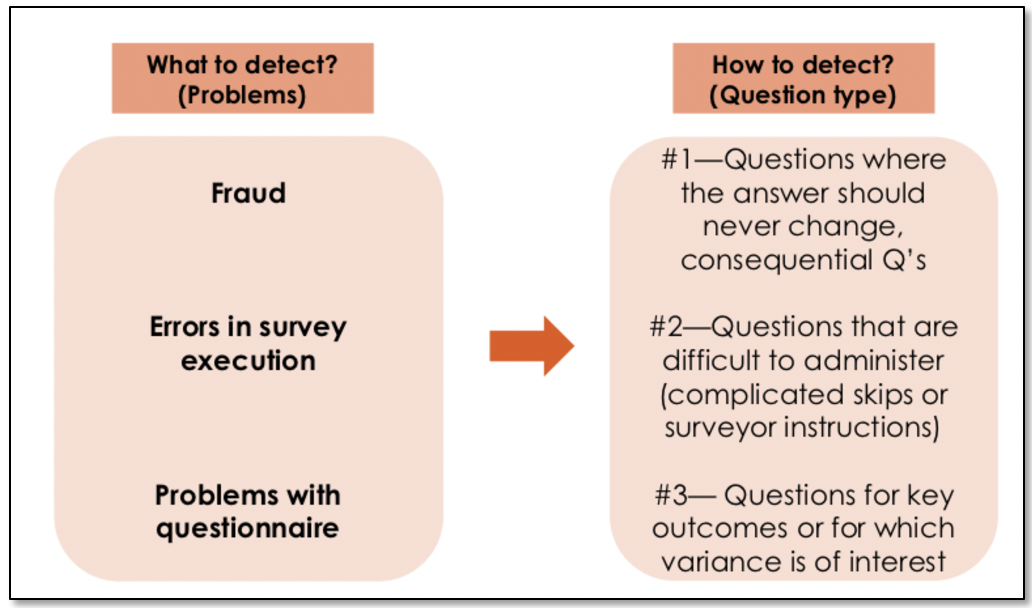
\includegraphics[width=75mm]{img/Quality}
	\end{figure}
	
\end{multicols}
\end{frame}


\begin{frame}[fragile]{3 lines of defense against low-quality data}
\begin{multicols}{2}	
	
	\begin{enumerate}[<default overlay specification>]
		\item<1> \textbf{Survey design}
				\newline - Use constraints and relevance in survey coding. Make sure questions are clear in English and survey language. Pilot survey effectively so team is well-practiced.
		\item<1> \textbf{Field management}
					\newline - Enumerators and managers “buy-in” to quality. Check in constantly and make team feel valued. Unless egregious/fraudulent, errors are yours. 
		\item<1> \textbf{High-frequency checks}
					\newline Demonstrate that quality. Catch key mistakes early. Visible performance metrics.
	\end{enumerate}
	
	\begin{figure}
		\centering
		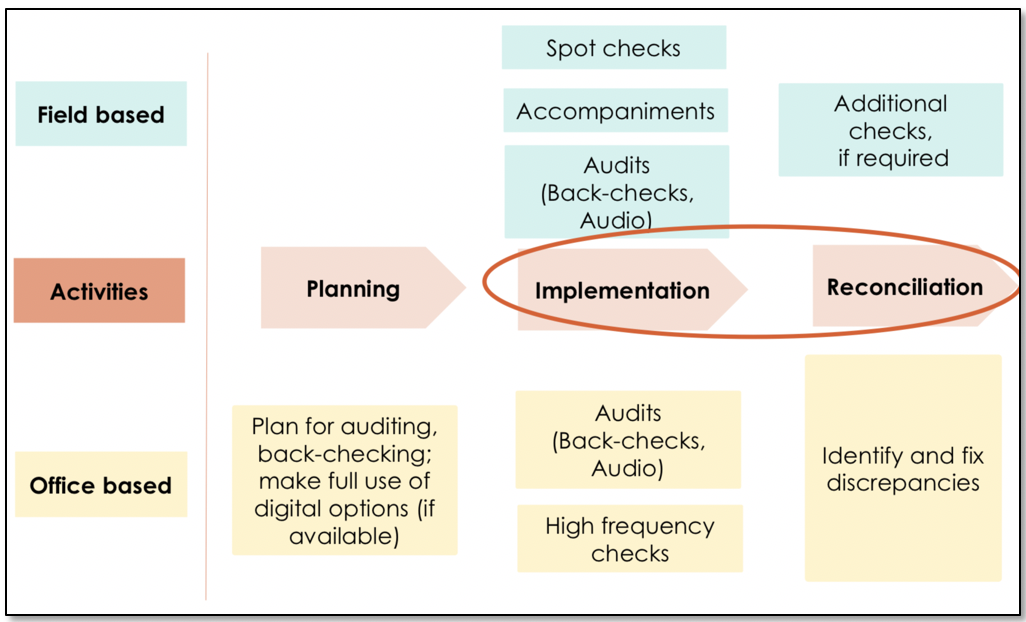
\includegraphics[width=65mm, right]{img/Quality2}
	\end{figure}
	
\end{multicols}
\end{frame}


\begin{frame}[fragile]{Well-coded surveys}
\begin{multicols}{2}	
	
	\begin{itemize}[<default overlay specification>]
		\item<1> Relevance fields and constraint fields in survey design can provide instant feedback to enumerators.
		\item<1> It also reminds them you care about this and have put in a lot of work to make it easy for them to do right!
	\end{itemize}
	
	\begin{figure}
		\centering
		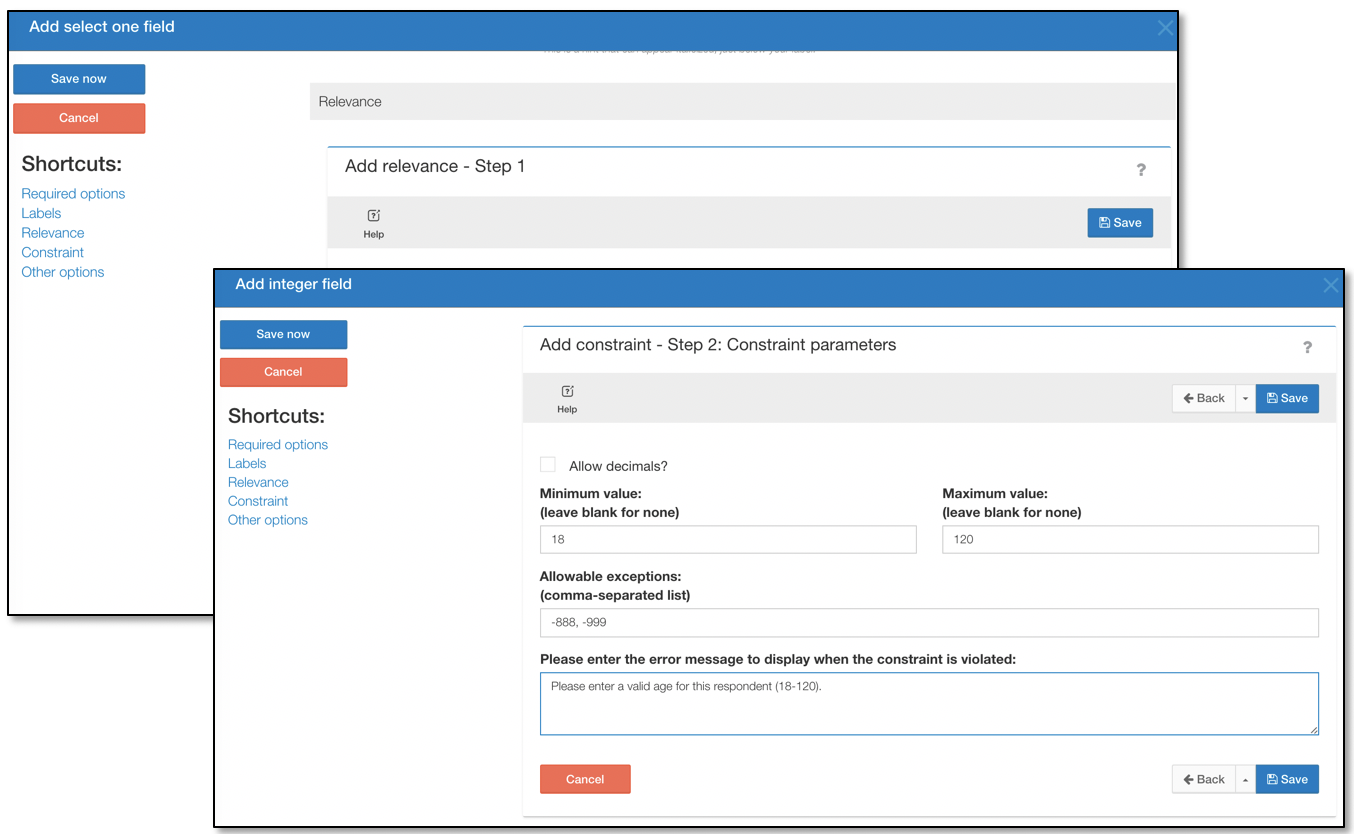
\includegraphics[width=70mm, right]{img/Survey}
	\end{figure}
	
\end{multicols}
\end{frame}


\begin{frame}[fragile]{3 lines of defense against low-quality data}
\begin{multicols}{2}	
	
	\begin{itemize}[<default overlay specification>]
		\item<1> Data entry starts with a page containing:
			\newline - Location/site ID [dropdown]
			\newline - Respondent ID [dropdown?]
			\newline - Enumerator ID [dropdown]
		\item<1> The next page preloads the corresponding names from those IDs based on the Universe and says: 
			\newline - You indicated that this survey was completed in [City Name], at [Clinic Name], with [Provider Name] by [SP Name]. Is that correct? (Answer: Yes/No)
		\item<1> Enumerator checks this against the written names on the assignments, if that exists, and reports back any inconsistency.
	\end{itemize}
	
	\begin{figure}
		\centering
		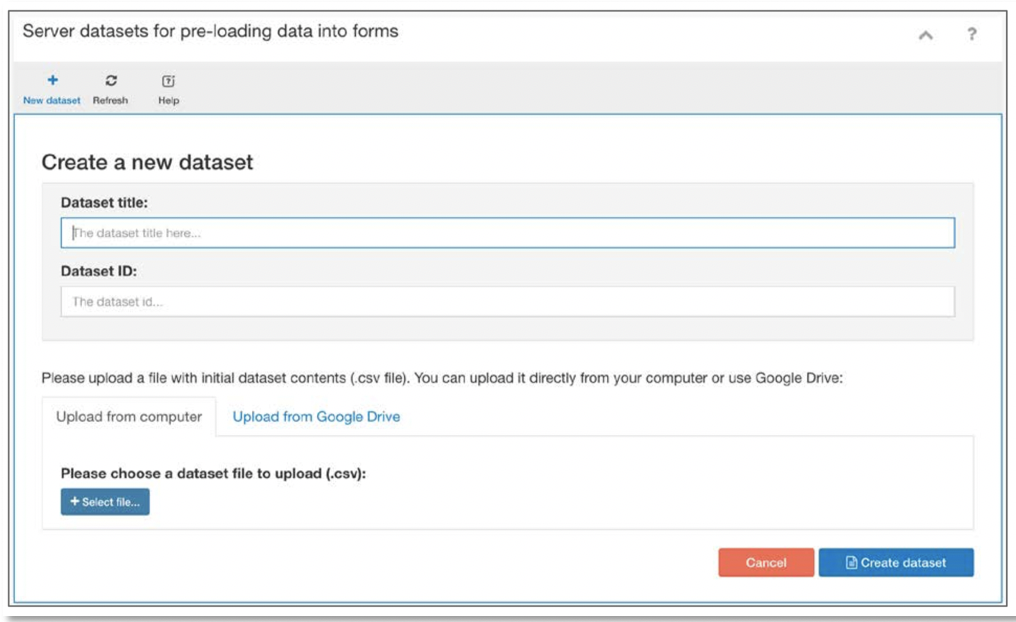
\includegraphics[width=65mm, right]{img/Survey2}
	\end{figure}
	
\end{multicols}
\end{frame}


\begin{frame}[fragile]{Key tool in survey design: tracking sheets}
\begin{multicols}{2}	
	
	\begin{itemize}[<default overlay specification>]
		\item<1> Data quality in the field is best supported by “continuous” accountability.
		\item<1> Tracking should be compared against the prepopulated list, if possible.
		\item<1> Survey tracking, if used, must be entered every day and are “core tasks”, not “in addition” to the survey work. 
	\end{itemize}
	
	\begin{figure}
		\centering
		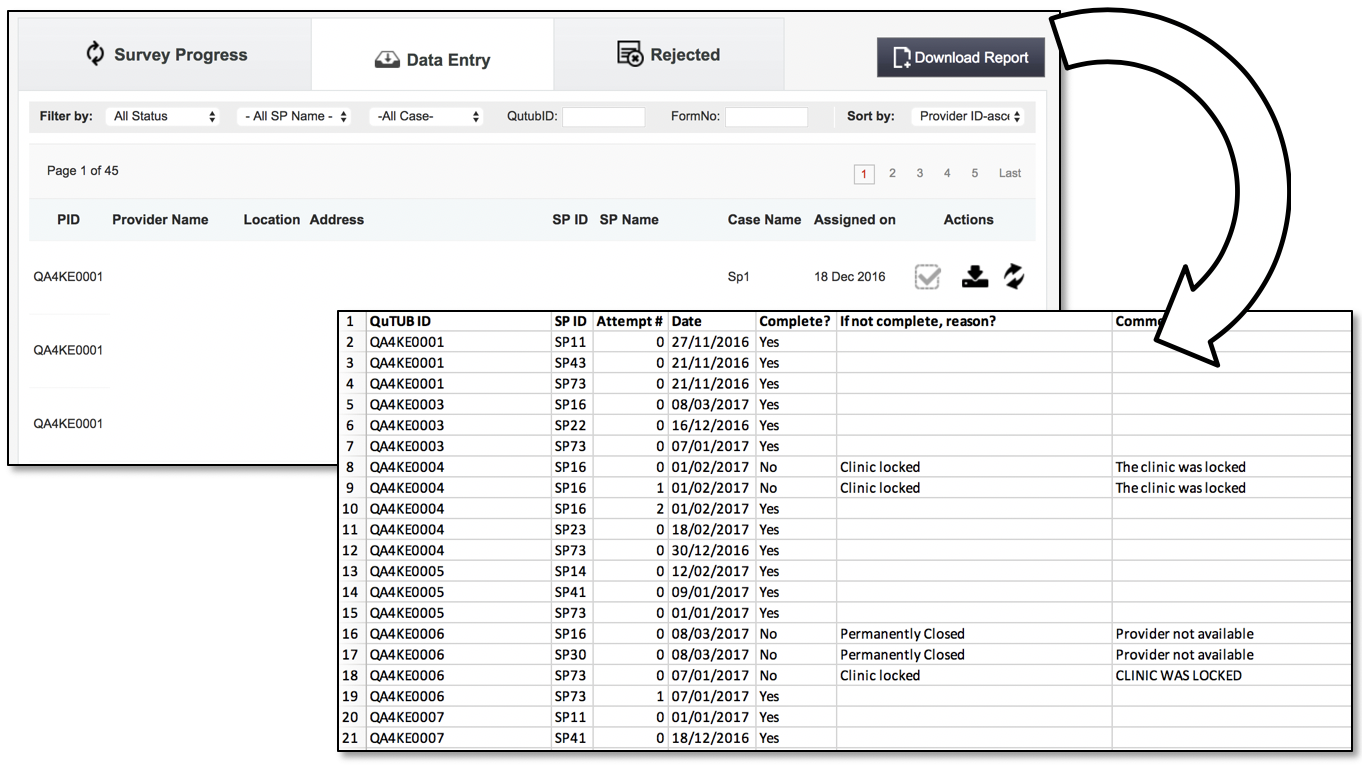
\includegraphics[width=65mm, right]{img/Survey3}
	\end{figure}
	
\end{multicols}
\end{frame}



\begin{frame}[fragile]{SurveyCTO allows “case management”}
\begin{multicols}{2}	
	
	\begin{itemize}[<default overlay specification>]
		\item<1> Surveys are pre-assigned to individuals (potentially also to enumerators).
		\item<1> Completion can be monitored in real-time against the preset list.
		\item<1> This works if you know the list of who should be interviewed (but not if you don’t).
	\end{itemize}
	
	\begin{figure}
		\centering
		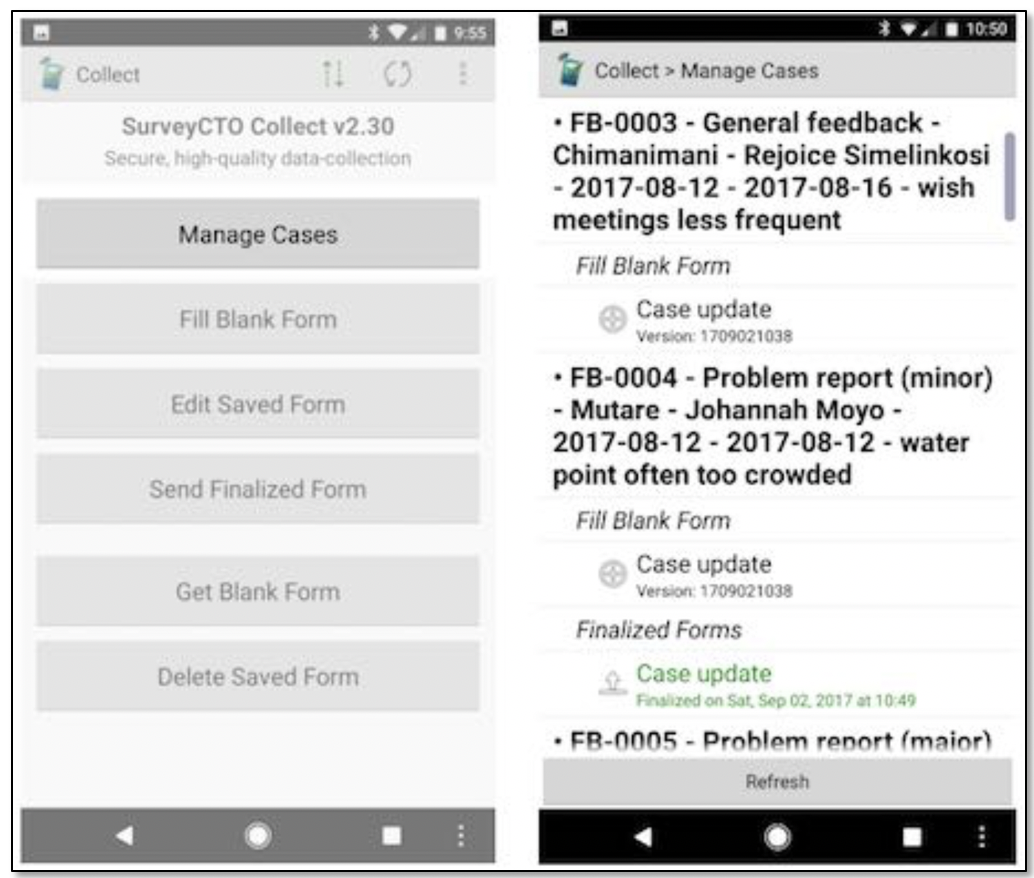
\includegraphics[width=65mm, right]{img/Survey4}
	\end{figure}
	
\end{multicols}
\end{frame}


\begin{frame}[fragile]{Reminder: Back-Check Surveys}
	
	\begin{itemize}[<default overlay specification>]
		\item<1> \textbf{ The answers are compared with the original survey}
			\newline - Every team and every surveyor must be back-checked as soon as possible, and regularly.
		\item<1> \textbf{ Should cover 1\% of sample, with 20\% being administered in the first 2 weeks of field work.}
			\newline - Random sub-sample. 
			\newline - Include missing respondents to verify that your team is not biasing your sample by not tracking hard to find respondents. 
			\newline - Observations flagged in other quality tests
		\leavevmode 	\newline - Surveys of enumerators who are suspected of cheating.
	\end{itemize}
	
\end{frame}


\begin{frame}{Back-Check Variables: use [bcstats]}

\begin{figure}
	\centering
	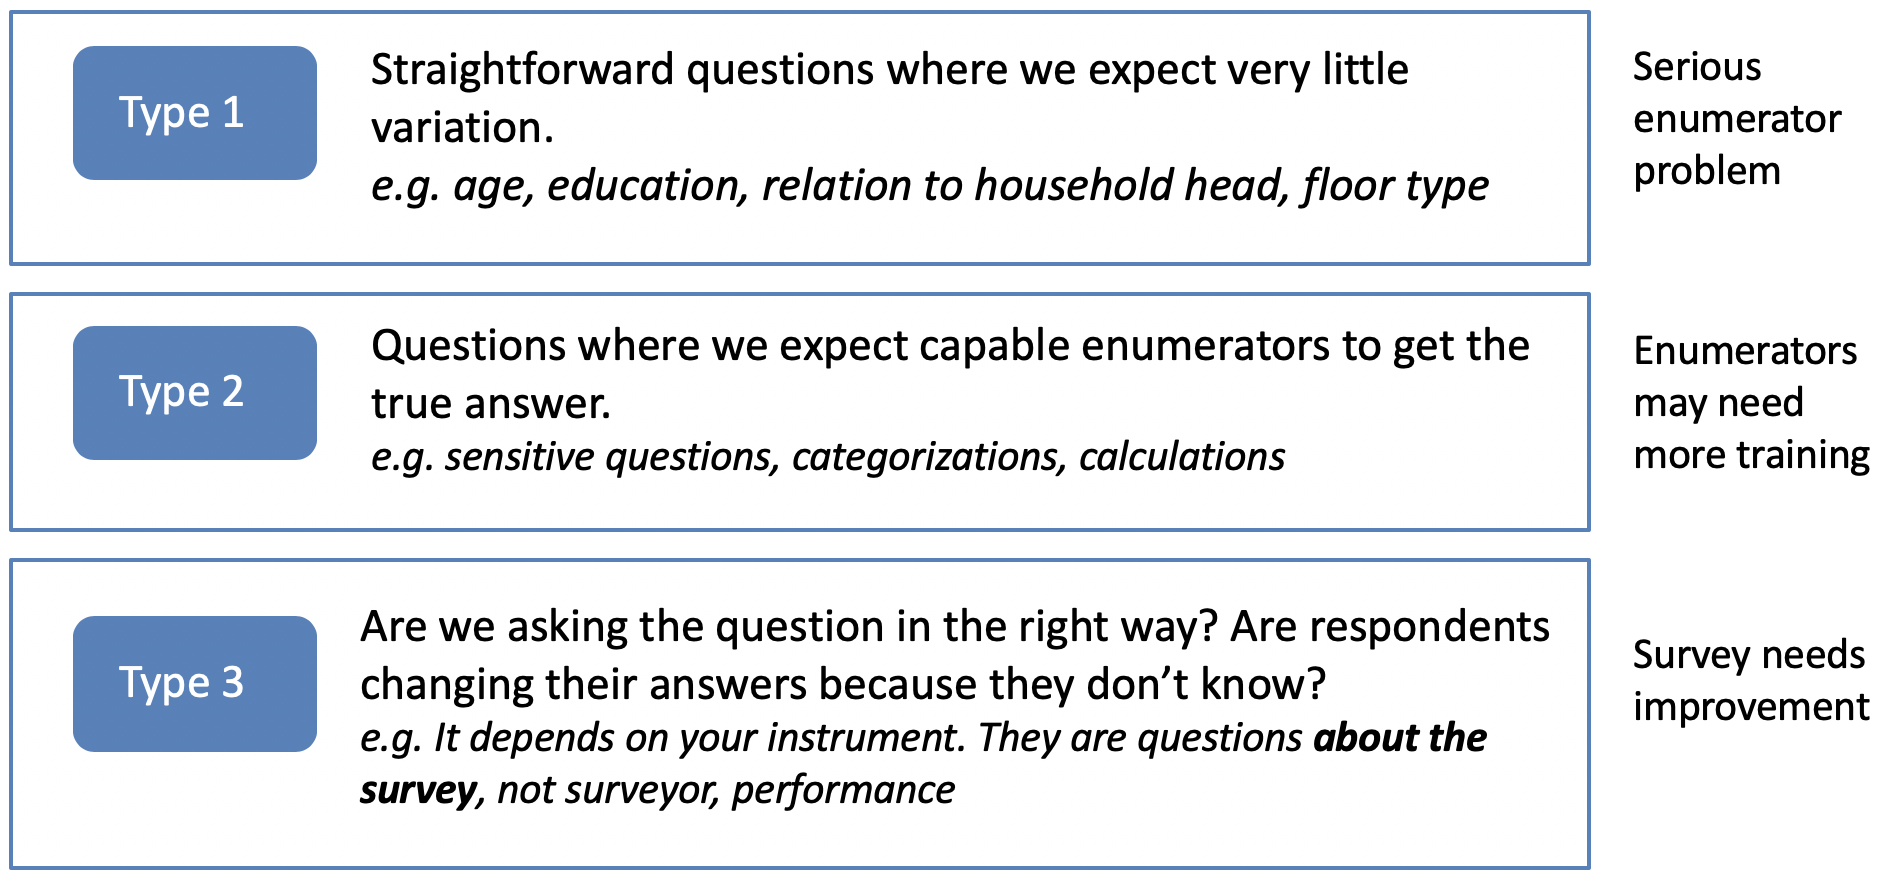
\includegraphics[width=\linewidth]{img/Backcheck}
\end{figure}

\end{frame}


\begin{frame}[fragile]{In the office: High-frequency checks}
\begin{multicols}{2}	
	
	\begin{itemize}[<default overlay specification>]
		\item<1> Done by you:
			\newline - Prepare code / instructions for HFCs before the survey goes to field.
			\newline - Monitor flags reporting and address in the field.
		\item<1> Done by the research assistant:
			\newline - Maintain HFC code. 
			\newline - Daily data download.
			\newline - Daily flags reporting. 
			\newline - This should be a one-click process.
	\end{itemize}
	
	\begin{figure}
		\centering
		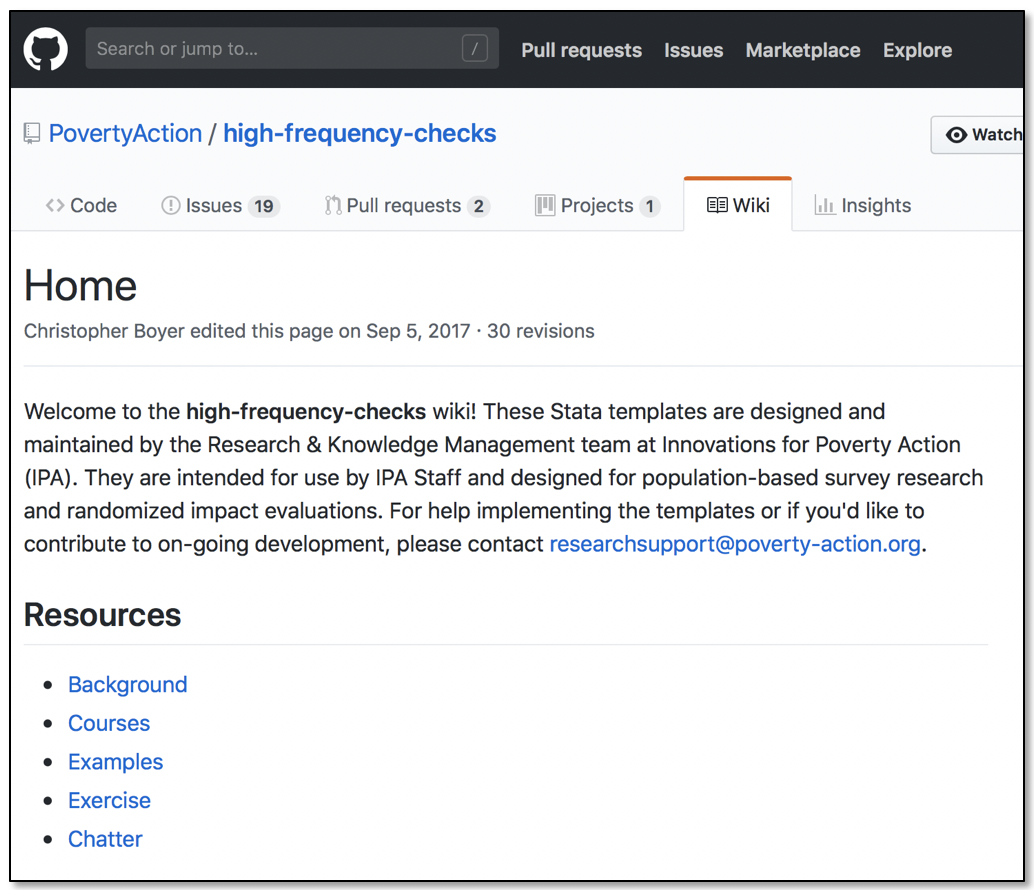
\includegraphics[width=65mm, right]{img/HFCs}
	\end{figure}
	
\end{multicols}
\end{frame}


\begin{frame}[fragile]{SurveyCTO allows tracking dashboards}
\begin{multicols}{2}	
	
	\begin{itemize}[<default overlay specification>]
		\item<1> \textbf{Examples}
		https://www.surveycto.com/best-practices/hacking-google-sheets-for-real-time-dashboards/
		https://www.surveycto.com/case-studies/monitoring-and-visualization/ 
	\end{itemize}
	
	\begin{figure}
		\centering
		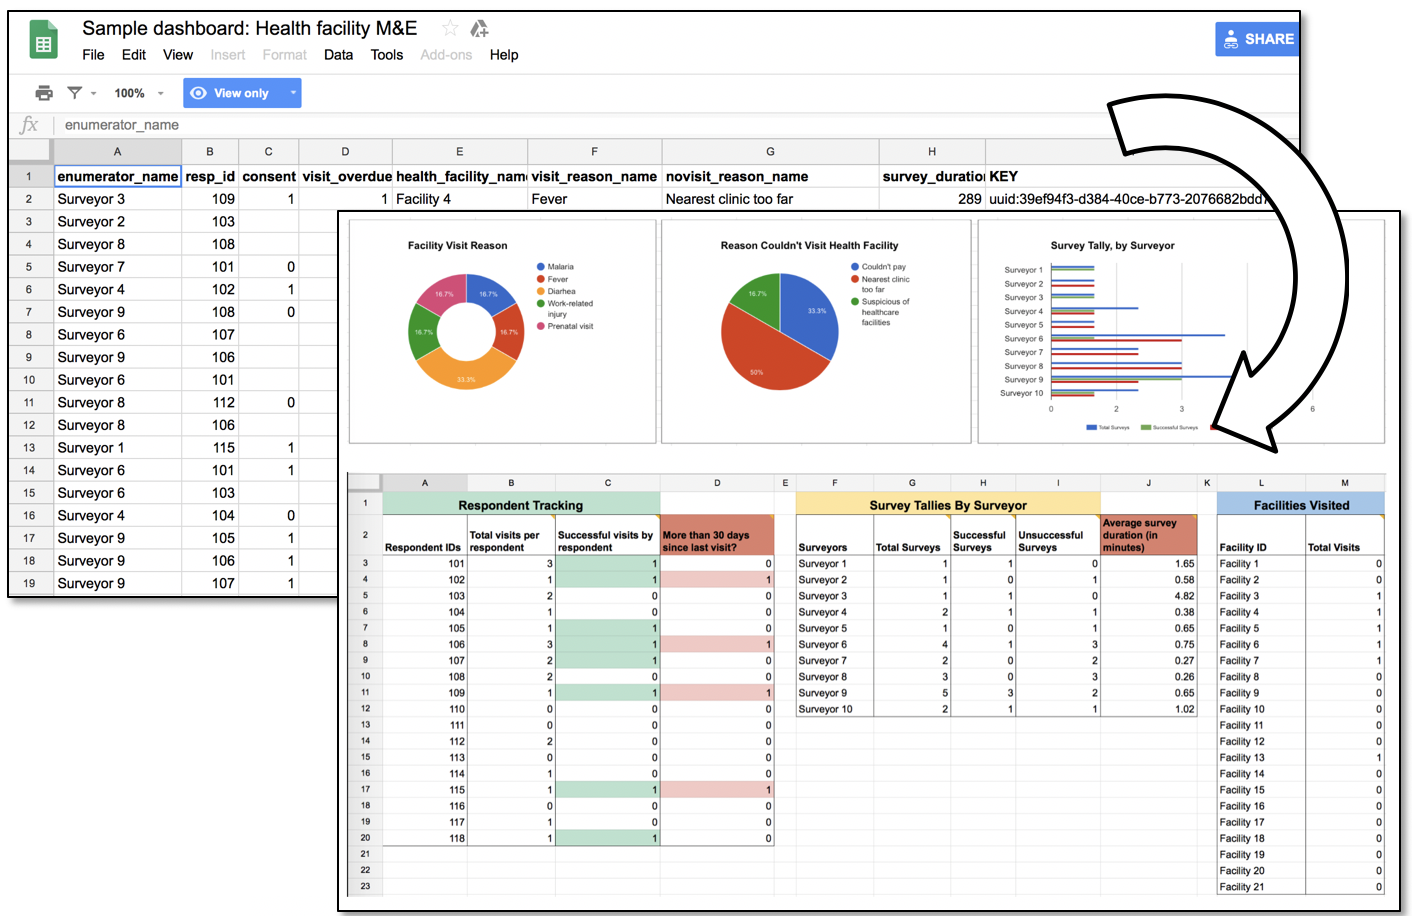
\includegraphics[width=75mm, right]{img/Dashboard}
	\end{figure}
	
\end{multicols}
\end{frame}


\begin{frame}[fragile]{SurveyCTO has new workflow tools for QA}
\begin{multicols}{2}	
	
	\begin{itemize}[<default overlay specification>]
		\item<1> Quality issues can be dealt with as they arise:
			\newline - Enumerator is consistently fast/slow.
			\newline - Back-check disagrees with survey
			\newline - Random resurveying
	\end{itemize}
	
	\begin{figure}
		\centering
		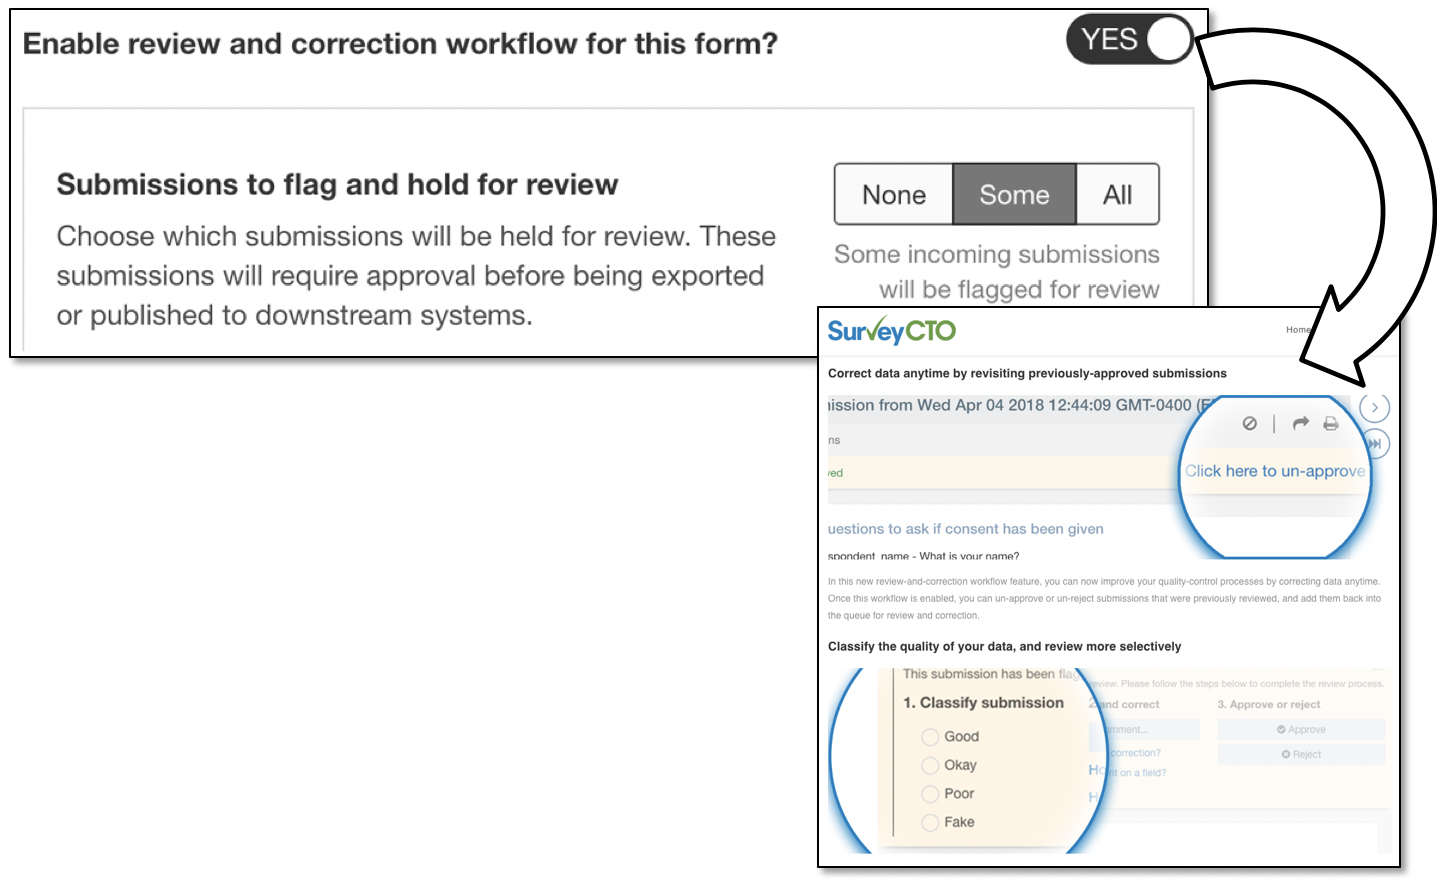
\includegraphics[width=70mm, right]{img/Workflow}
	\end{figure}
	
\end{multicols}
\end{frame}


\begin{frame}[fragile]{Daily downloads of data support routine checks}
\begin{multicols}{2}	
	
	\begin{itemize}[<default overlay specification>]
		\item<1> \textbf{Enumerator checks}
			\newline - Check the percentage of “don’t know” and “refusal” responses by enumerator.
			\newline - Check the distribution of responses for key questions by enumerator.
			\newline - Check the number of surveys per day by enumerator.
			\newline - Check the average interview duration by enumerator.
			\newline - Check the duration of consent by enumerator.
		\item<1> \textbf{ Project checks}
			\newline - Overall survey progress relative to planned sample.
			\newline - Summaries of key research variables.
			\newline - Two-way summaries of survey variables by demographic/geographic characteristics.
			\newline - Attrition rates by type and treatment status.
			\newline - Maps/GIS: all observations where they’re meant to be?
	\end{itemize}
	
\end{multicols}
\end{frame}


\begin{frame}{SCTO can also automate some of these checks}

\begin{figure}
	\centering
	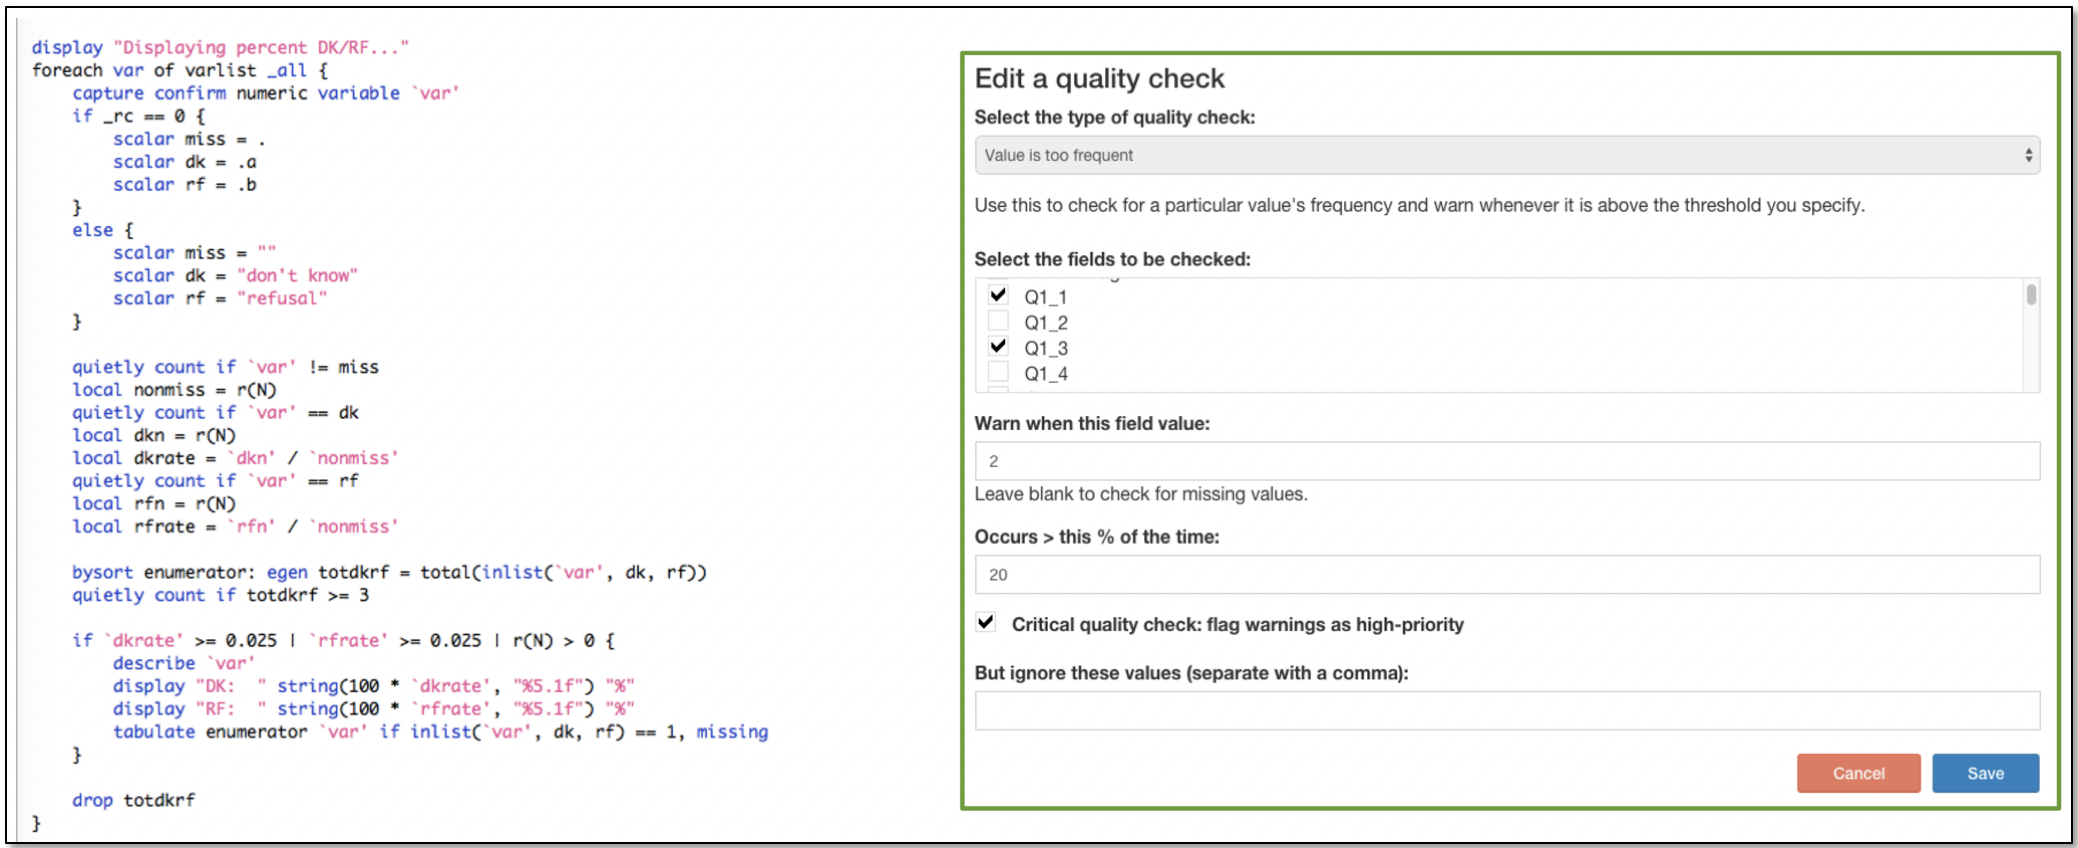
\includegraphics[width=\linewidth]{img/HFCs2}
\end{figure}

\end{frame}


%%%%%%%%%%%%% heading of section 1 %%%%%%%%%%%%%%%%%%%%%%%
\sectionpic{Treatment Monitoring}{img/section_slide}

\begin{frame}{What is treatment monitoring?}

	\begin{itemize}[<default overlay specification>]
	\item<1>   Ensuring that individuals to which treatment is assigned actually receive treatment (or at least an offer of treatment) and that control households do not receive treatment.
	\item<1>   Treatment contamination is when some of the control group receives the treatment.
	\item<1> It should be reduced to as great an extent as possible.
\end{itemize}

\end{frame}


\begin{frame}{Example: Savings, Grants, Training}
	
	\begin{itemize}[<default overlay specification>]
	\item<1>   In the context of new rural roads, we study the impact of complementary interventions for increasing productivity:
	\item<1>  Mechanisms for facilitating access to capital for investment . . .
			\begin{figure}
				\centering
				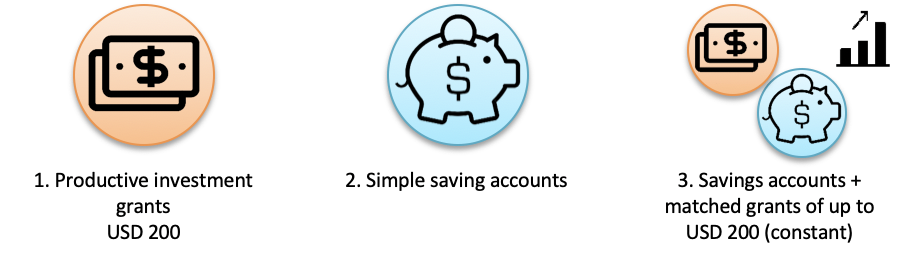
\includegraphics[width=50mm]{img/Monitoring}
			\end{figure}
	\item<1>  Developing the soft skills necessary to be a successful entrepreneur.
			\begin{figure}
				\centering
				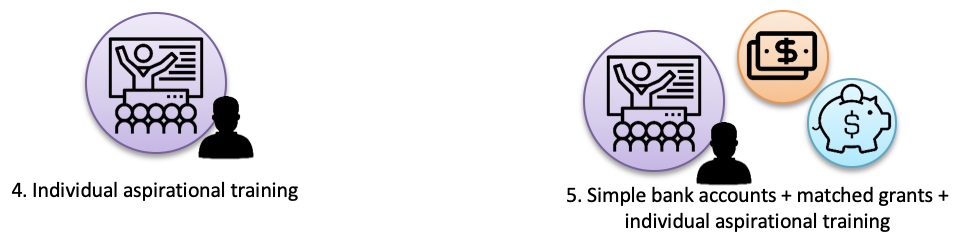
\includegraphics[width=50mm]{img/Monitoring2}
			\end{figure}
	\end{itemize}

\end{frame}


\begin{frame}{Savings accounts}

	\begin{figure}
		\centering
		
\includegraphics[width=\linewidth]{img/Savings}
	\end{figure}

\end{frame}

\begin{frame}{Personal initiative training}

	\begin{figure}
		\centering
		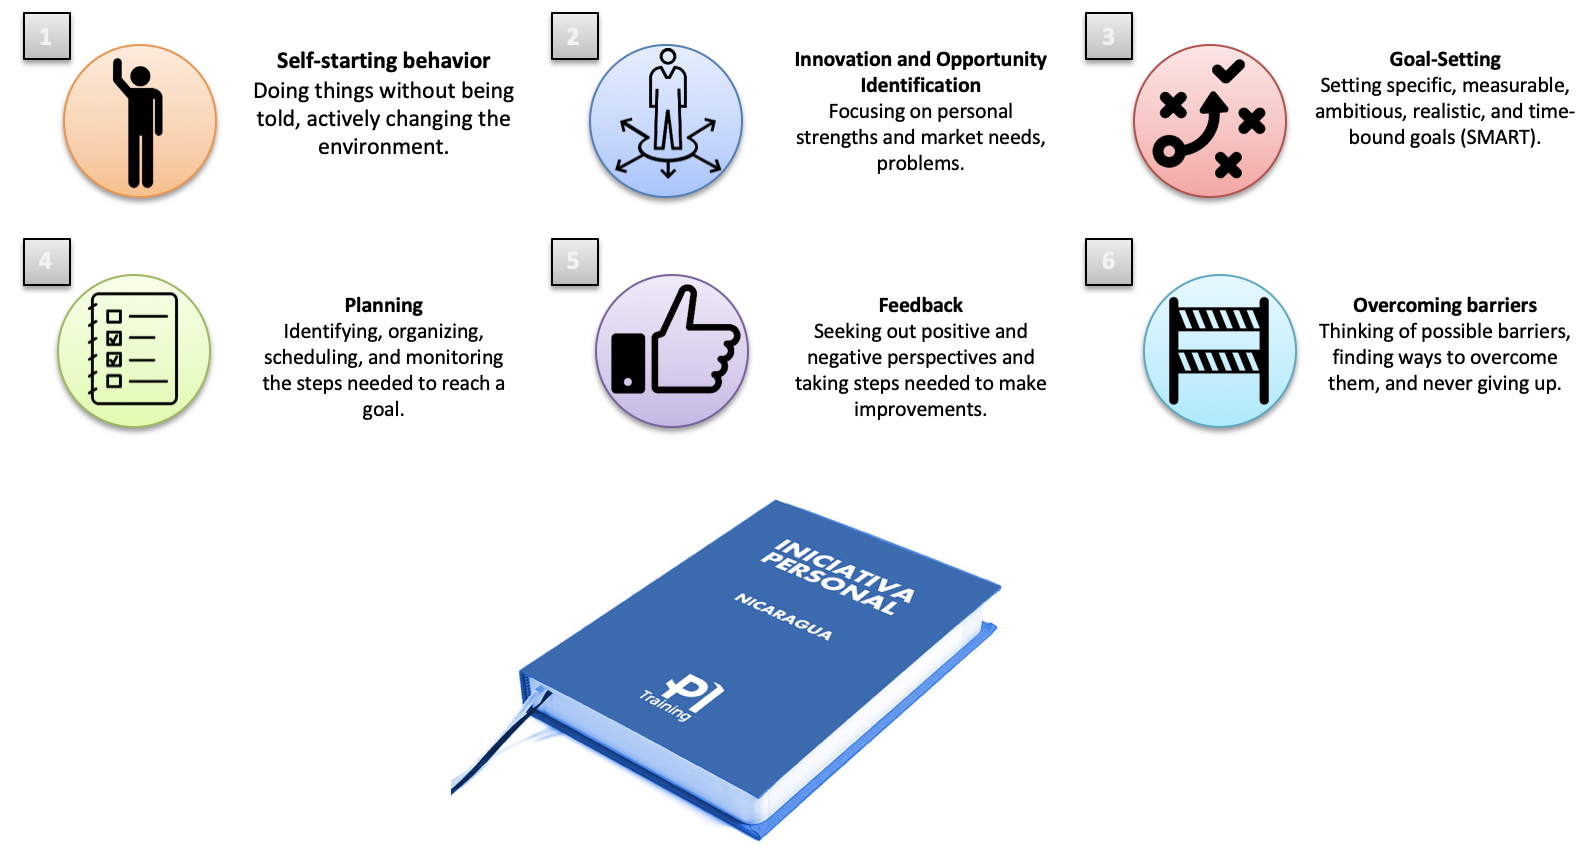
\includegraphics[width=\linewidth]{img/Training}
	\end{figure}

\end{frame}


\begin{frame}{How can we monitor treatment fidelity?}

\begin{itemize}[<default overlay specification>]
	\item<1>   Physical checks (from the field)
		\newline Performance of random physical in-person checks to ensure treatment applied as stated in IE protocol to units selected for treatment.
	\item<1> Administrative data (from the office)
		\newline Checking attendance, account records to ensure treatment applied only to treatment HH and not to the control group.
\end{itemize}

\end{frame}


\begin{frame}{Physical checks}

\begin{itemize}[<default overlay specification>]
	\item<1>   Ensure treatment is offered:

		\leavevmode 		\newline - to the correct households (complicated by poor geospatial data, names as written on official identity cards, i.e., “El Loco”)
		\newline - in the following order: HH head, spouse, oldest child above 18
		\newline -  according to the script to the extent possible so that all training offers are the same
		\newline - using marketing materials as planned
	\item<1> For the training, could have checked to ensure participants were only those to whom treatment was offered
\end{itemize}

\end{frame}


\begin{frame}{Administrative data}

\begin{itemize}[<default overlay specification>]
	\item<1>   Training

	\leavevmode 		\newline - Check attendance and pre-/post- tests to ensure that only HH to which treatment was offered are attending training.
	\item<1> Savings accounts
		\newline - Check accounts opened to ensure account opener related in some way to the household (based on BL data).
		\newline -  Correct functioning of matching mechanism (i.e., individuals achieving pre-determined savings goals receive match).
		\newline - After each match period, commercial bank sent Excel with accounts, savings behavior, and amount of match (if any) to be received by account-holders.
		\newline - Important to ensure that IE team and implementing partner (in this case, a bank) on the same page and that treatment is not applied incorrectly.
\end{itemize}

\end{frame}

\begin{frame}{Other field challenges}

\begin{itemize}[<default overlay specification>]
	\item<1>   Re: the training, implementing NGO found that allowing community leaders to participate in training would increase take-up of community members.
		\newline -  But concerns over spillovers (i.e., control HH in communities in which leaders participate may benefit from the training in ways in which control HH in communities in which leaders do not).
		\newline - Ultimately, have to weigh potential for spillovers against possibility of reduced take-up.
\end{itemize}

\end{frame}

\begin{frame}{Other field challenges}

\begin{itemize}[<default overlay specification>]
	\item<1>   Two implementing organizations, each of which offered treatment without coordinating with the other.
	\item<1>  NGO did not know of bank’s presence and vice versa.
	\item<1> Led to confusion and mistrust on the part of community members directed at both implementers.
	\item<1> In the case of the combined training + matched grant treatment, led to reduced take-up: HH that had accepted the training, but after the account offer elected not to participate in the training (bank’s have a really bad rep in Nicaragua).
\end{itemize}

\end{frame}

\begin{frame}{Bottom line}

\begin{itemize}[<default overlay specification>]
	\item<1>  Things are going to go wrong!
	\item<1>  Plan as much as you can.
	\item<1> Establish good communication with your team (internally, at the WB, as well as with implementing partners).
	\item<1> Keep calm and . . . resolve issues as quickly and as effectively as possible
\end{itemize}

\end{frame}

%%%%%%%%%%%%%%%%%%%%%%%%%%%%%%%%%%%%%%%%%%% Final thougts section
\begin{frame}{Conclusion}

Thank You!

\vspace{20mm}
For more information or further questions please contact:
\newline Benjamin Daniels (\url{bdaniels@worldbank.org }) 
\end{frame}

%%%%%%%%%%%%%%%%%%%%%%%%%%%%%%%%%%%%%%%%%%% The End
\sectionpic{The End}{img/section_slide}






\end{document} 